% Fichier LaTeX enrichi avec images UPDF
% Exercice 1 - Amérique du Nord ^
% 20 points

\documentclass[12pt]{article}
\usepackage[utf8]{inputenc}
\usepackage[T1]{fontenc}
\usepackage[french]{babel}
\usepackage{graphicx}
\usepackage{amsmath}
\usepackage{amssymb}
\usepackage{geometry}
\geometry{a4paper, margin=2cm}

\begin{document}

\section*{Exercice 1 (20 points)}

% Images de l'exercice
\begin{center}
\includegraphics[width=0.8\textwidth]{images/dnb_2025_06_ameriquenord_1_Image_003.gif}
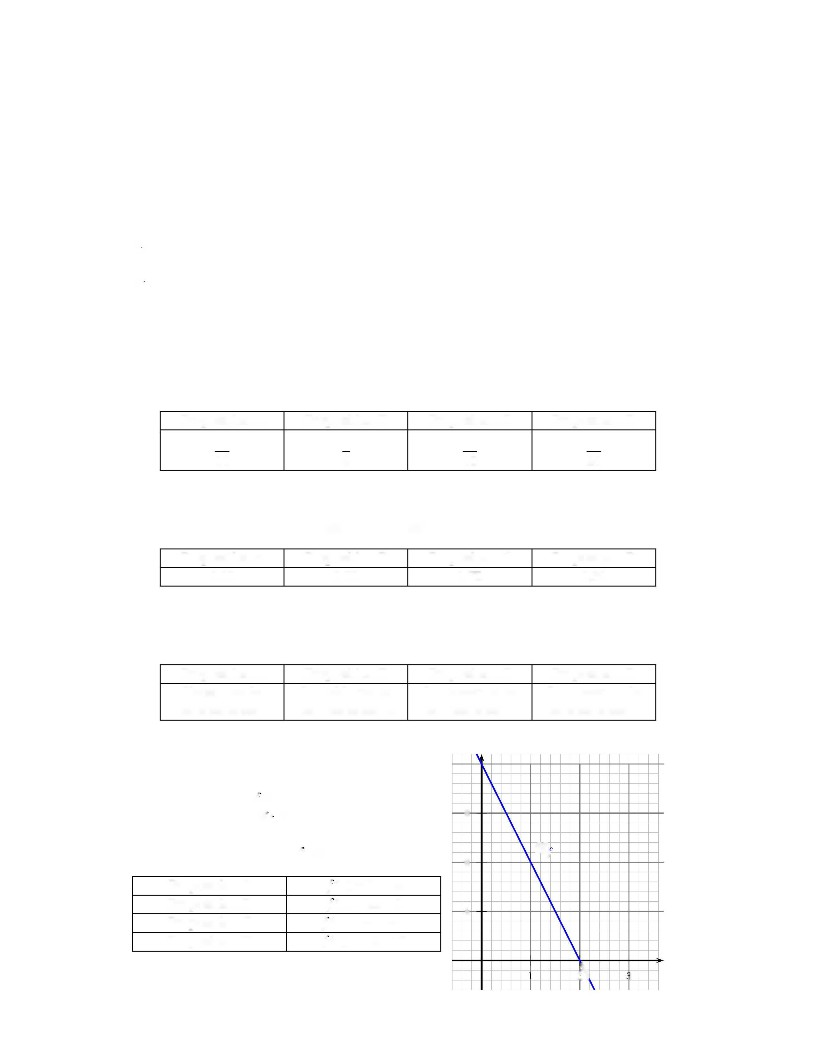
\includegraphics[width=0.8\textwidth]{images/dnb_2025_06_ameriquenord_1_Image_032.jpg}
\end{center}

\begin{enumerate}
\item Quelle est la moyenne des tailles des élèves de cette classe ?

\item Quelle est la médiane des tailles des élèves de cette classe ?

\end{enumerate}

\end{document}
